% Befehl \fibelvorstellung: Erstellt die Vorstellung eines FSlers mit Bild
%	Parameter #1: Bild (wrapfigure)
%	Parameter #2: Text
\newcommand{\fibelvorstellung}[2]{%
	\begin{minipage}{\columnwidth}
		% Kein Abstand vor bzw. nach Bildern bei wrapfigure
		\setlength{\intextsep}{0cm}
		% geringfügiger Abstand zwischen Paragraphen
		\setlength{\parskip}{0.5ex}
		#1
		#2
		\vspace{0.5ex}
	\end{minipage}
	
	\vspace{5ex plus 2ex minus 1ex}
}
\newlength{\fibelstdlen}
\setlength{\fibelstdlen}{3.7cm}

\section{Der Fachschaftsrat~(FSR) Physik stellt sich vor}
\begin{multicols}{2}
\small

\fibelvorstellung{
	\begin{wrapfigure}{r}{0cm}
		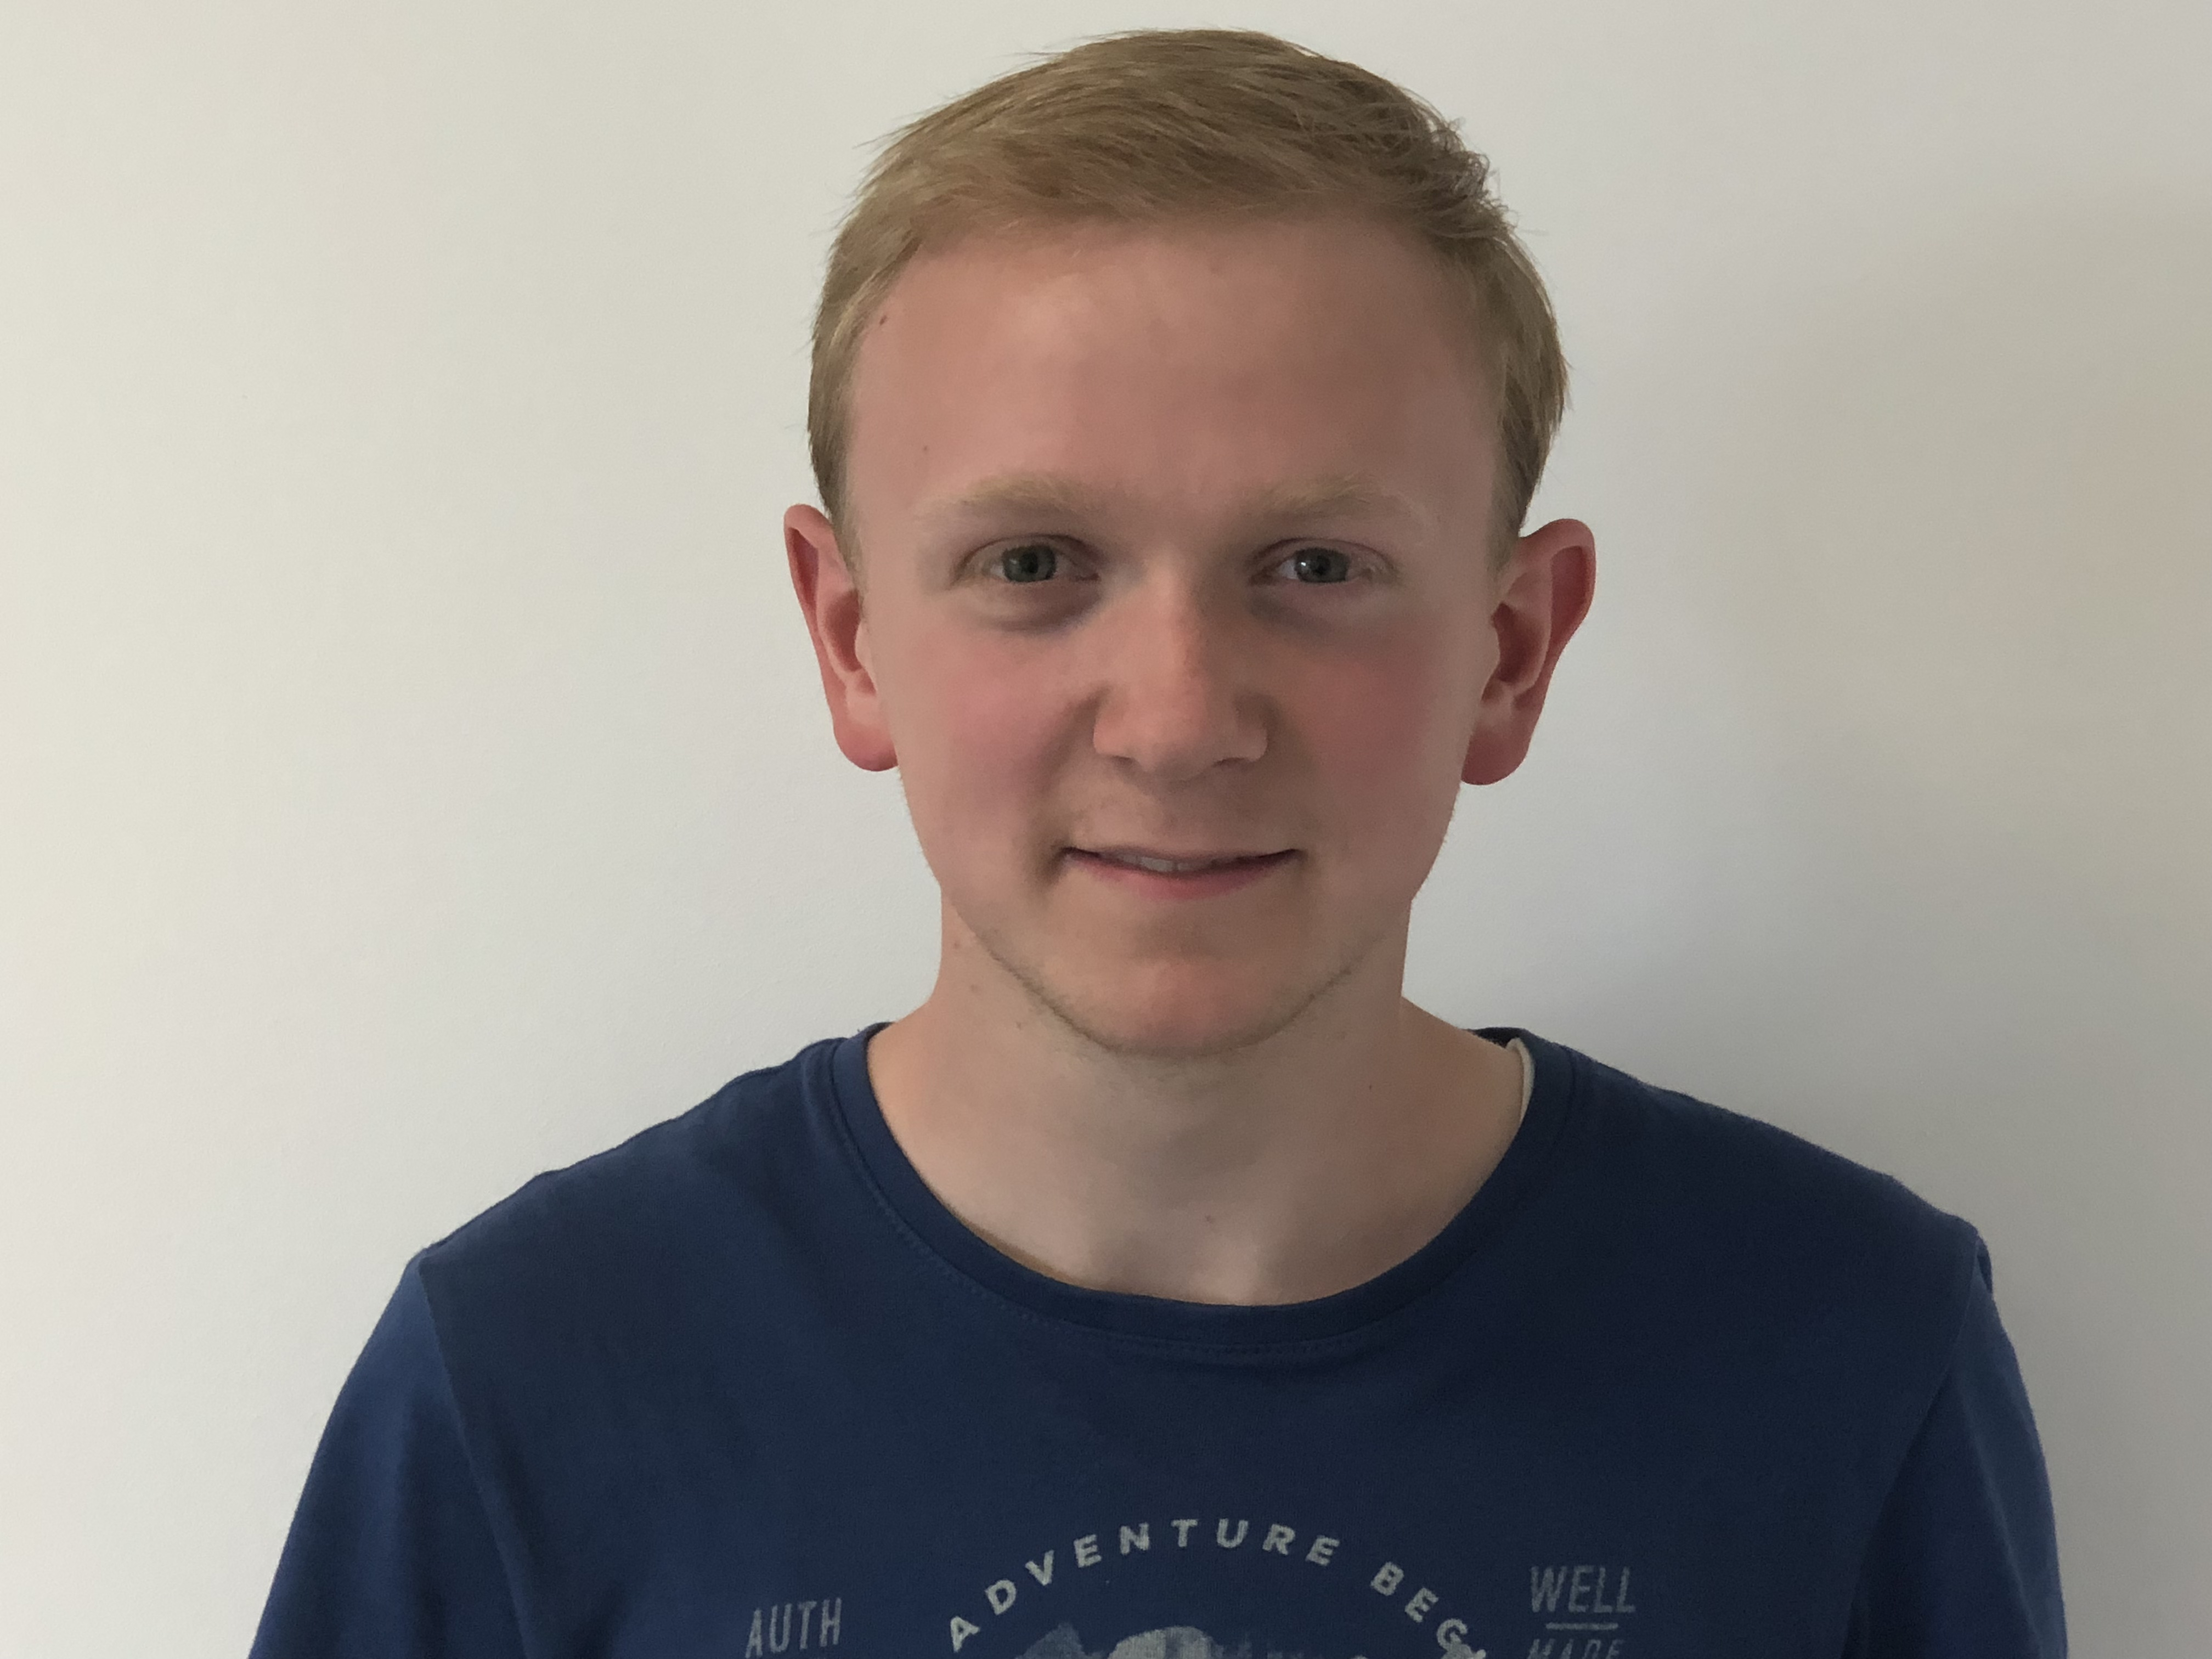
\includegraphics[width=\fibelstdlen]{res/vorstellungsfotos/tim_stellhorn.JPG}
	\end{wrapfigure}
}
{Hey Leute, ich bin Tim und studiere seit 4 Semestern Physik mit Nebenfach Informatik. Ich kann euch nur sagen, lasst euch auf keinen Fall von einem vielleicht etwas schwierigen Einstieg verunsichern, das wird schon. Doch erstmal möchte ich euch noch viel Spaß in der O-Woche wünschen. Und wenn ihr Lust habt, dann schaut mal beim Spieleabend der Fachschaft vorbei, vielleicht sieht man sich da ja wieder ;-)}


\fibelvorstellung{
	\begin{wrapfigure}{l}{0cm}
		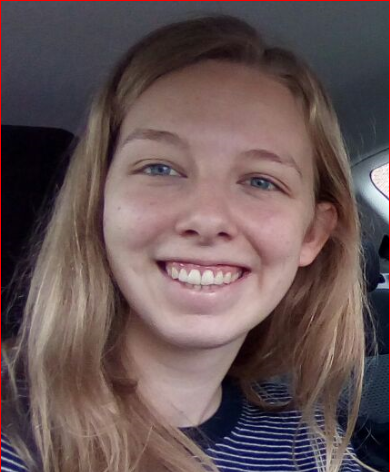
\includegraphics[width=\fibelstdlen]{res/vorstellungsfotos/anna_niemann_cropped.PNG}
	\end{wrapfigure}
}
{Hey, ich heiße Anna. Mit Fragen zum Studium oder Rund um Münster könnt ihr euch
	natürlich gerne an mich wenden. Ansonsten wünsche ich euch erstmal einen guten
	Start ins Studium:)
}
\vspace{1cm}

\fibelvorstellung{
	\begin{wrapfigure}{r}{0cm}
		\includegraphics[width=\fibelstdlen]{res/vorstellungsfotos/benedikt_bieringer.png}
	\end{wrapfigure}
}
{Hallo zusammen! Mein Name ist Benedikt. In der Fachschaft beschäftige ich mich unter anderem mit Computergrafik/Design. Programmieren und Schwimmen sind nur zwei meiner weiteren Freizeitbeschäftigungen. In meinen mittlerweile schon 8~Semestern Fachschafts- und Studienerfahrung kann ich euch aber auch bei einer ganzen Reihe weiterer Fragen weiterhelfen.
}

\fibelvorstellung{
	\begin{wrapfigure}{l}{0cm}
		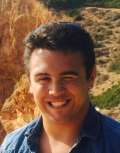
\includegraphics[width=\fibelstdlen]{res/vorstellungsfotos/fernando_romahn}
	\end{wrapfigure}
}
{Hey Leute, ich bin Fernando (der Name ist ostfriesisch auszusprechen). Zumeist bin ich ein ruhiger und gut gelaunter Typ (außer bei Mario Kart, da kenne ich keine Freunde). Bei Fragen, Problemen oder Lobeshymnen auf mich habe ich immer ein offenes Ohr für euch :)
}

\fibelvorstellung{
	\begin{wrapfigure}{l}{0cm}
		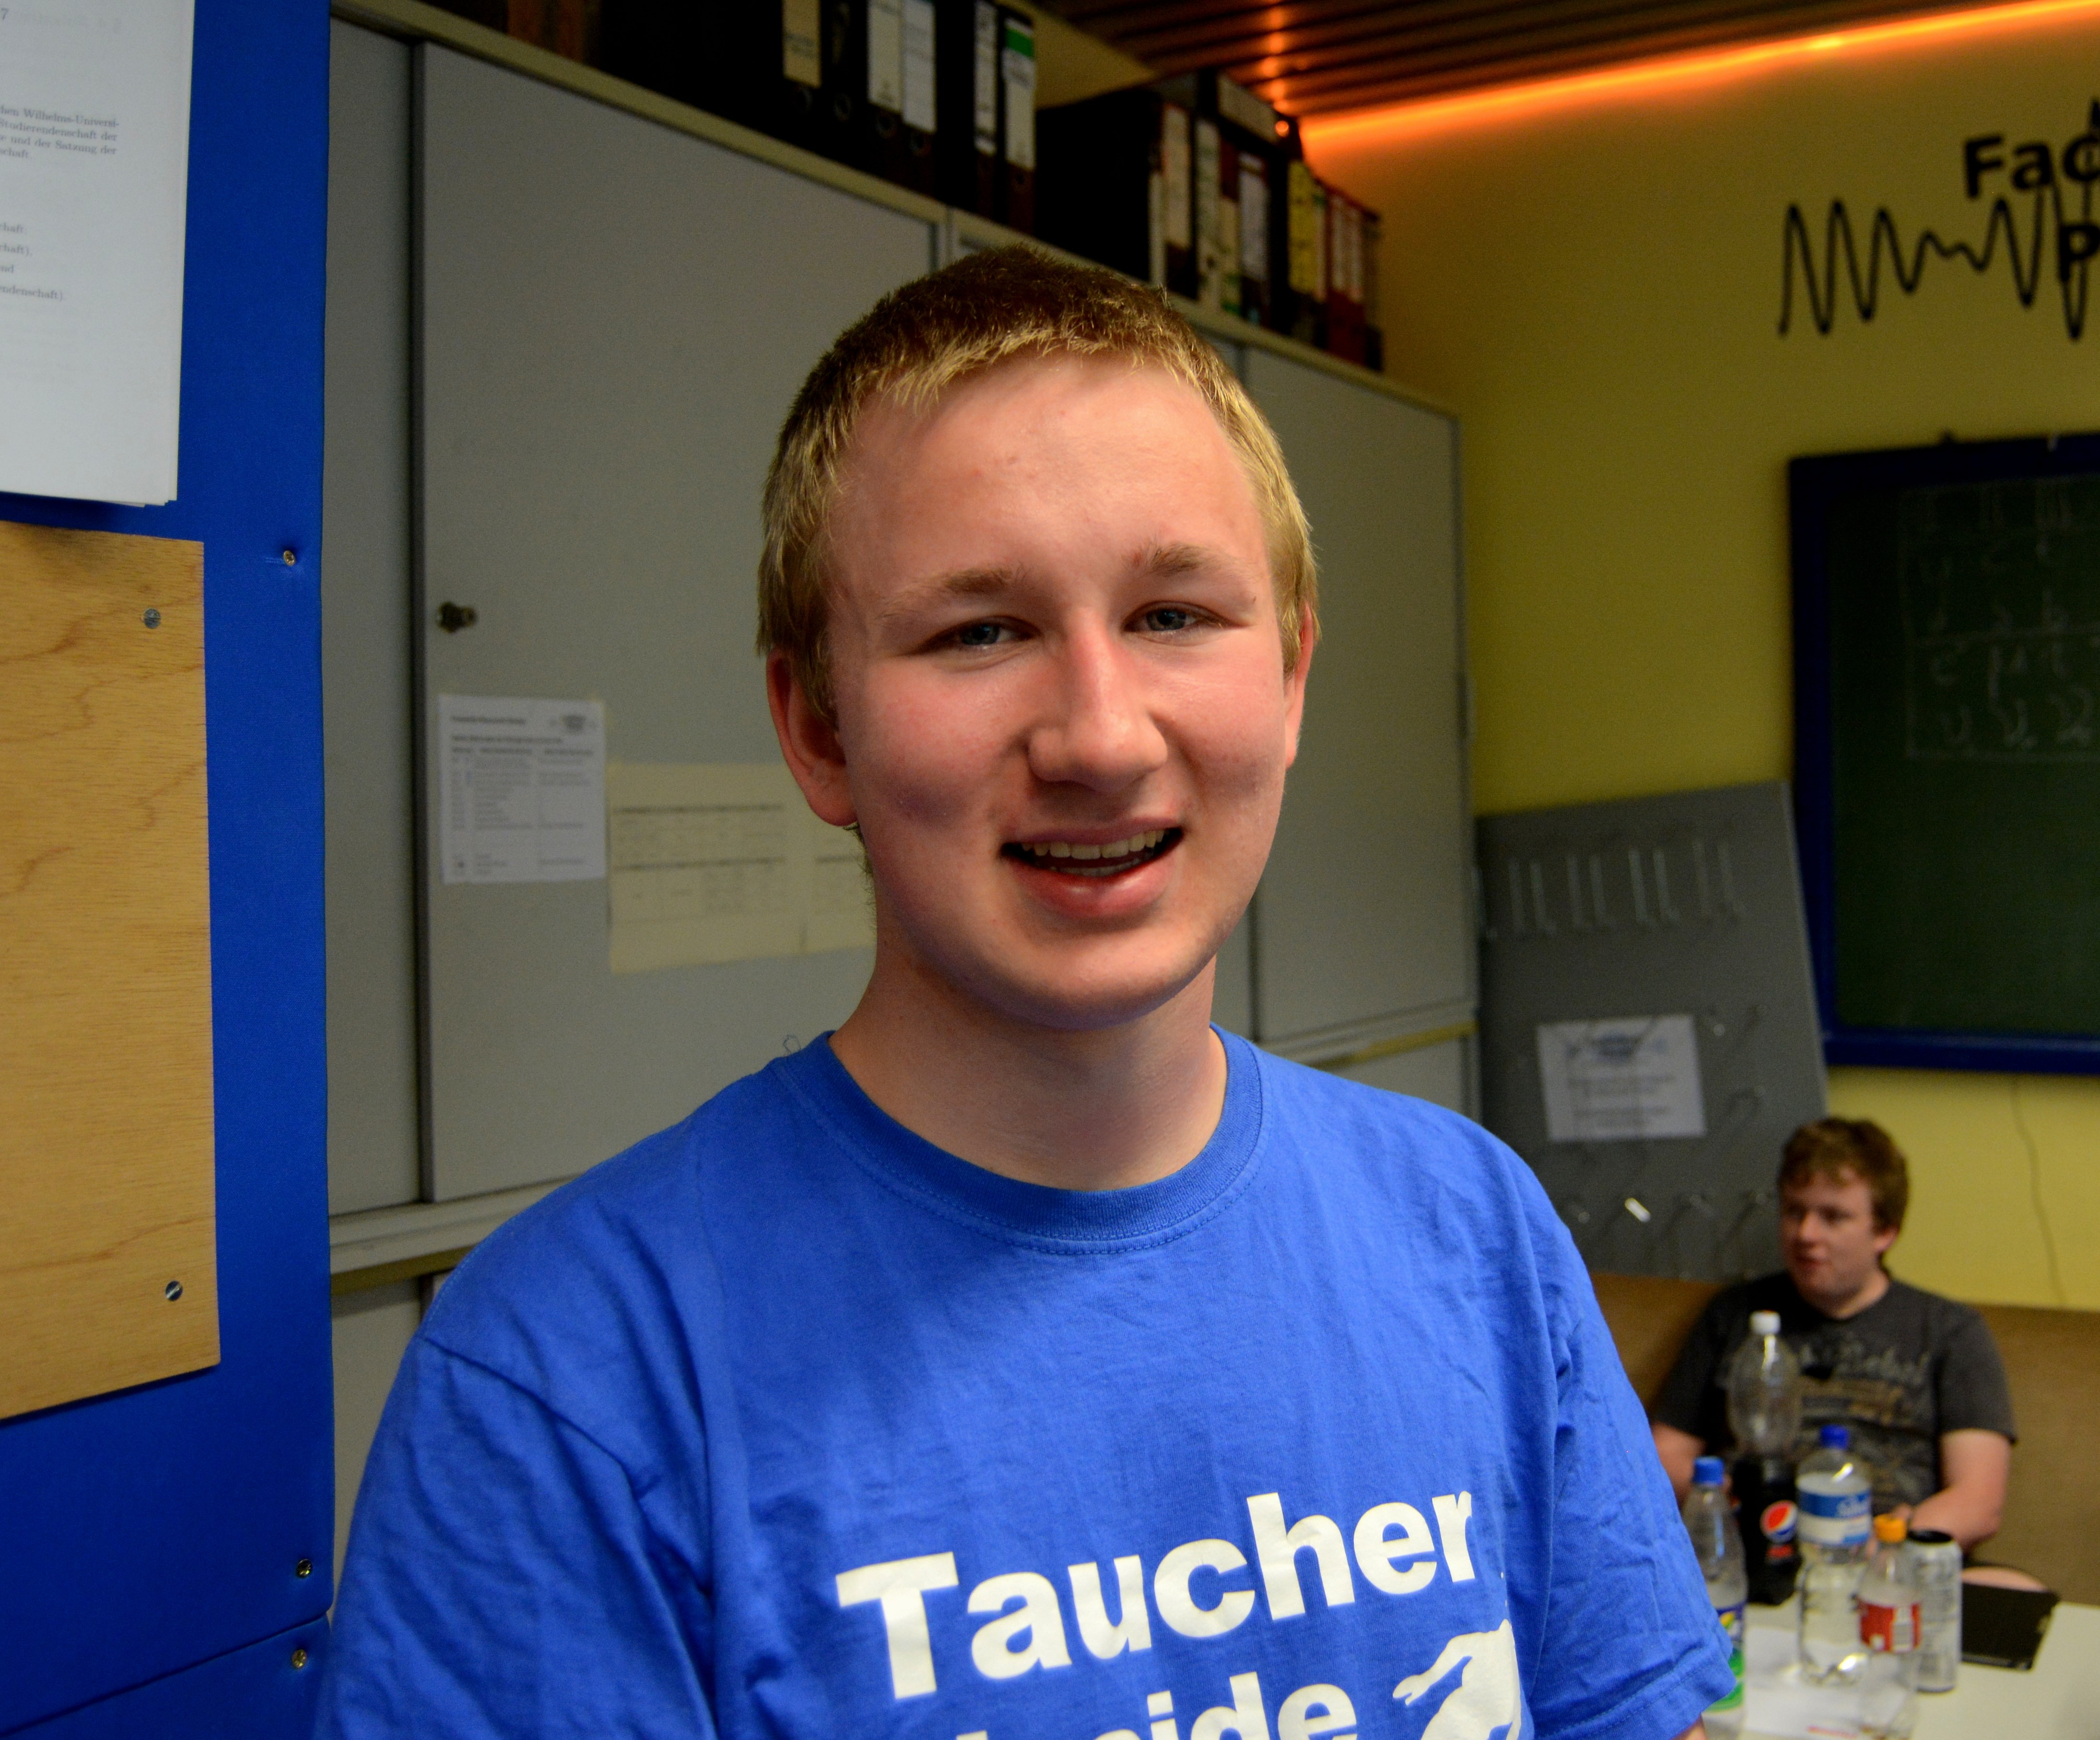
\includegraphics[width=\fibelstdlen]{res/vorstellungsfotos/hauke_hawighorst_neu.jpg}
	\end{wrapfigure}
}
{Moin, ich bin Hauke und seit 2016 an der Uni und in der Fachschaft. Nach dem ich letztes Jahr als Erasmusstudent in Sevilla (Spanien) war, werde ich dieses Jahr wieder die Evaluation der Lehre betreuen. Euch ein herzliches Willkommen in Münster! 
}

\fibelvorstellung{
	\begin{wrapfigure}{r}{0cm}
		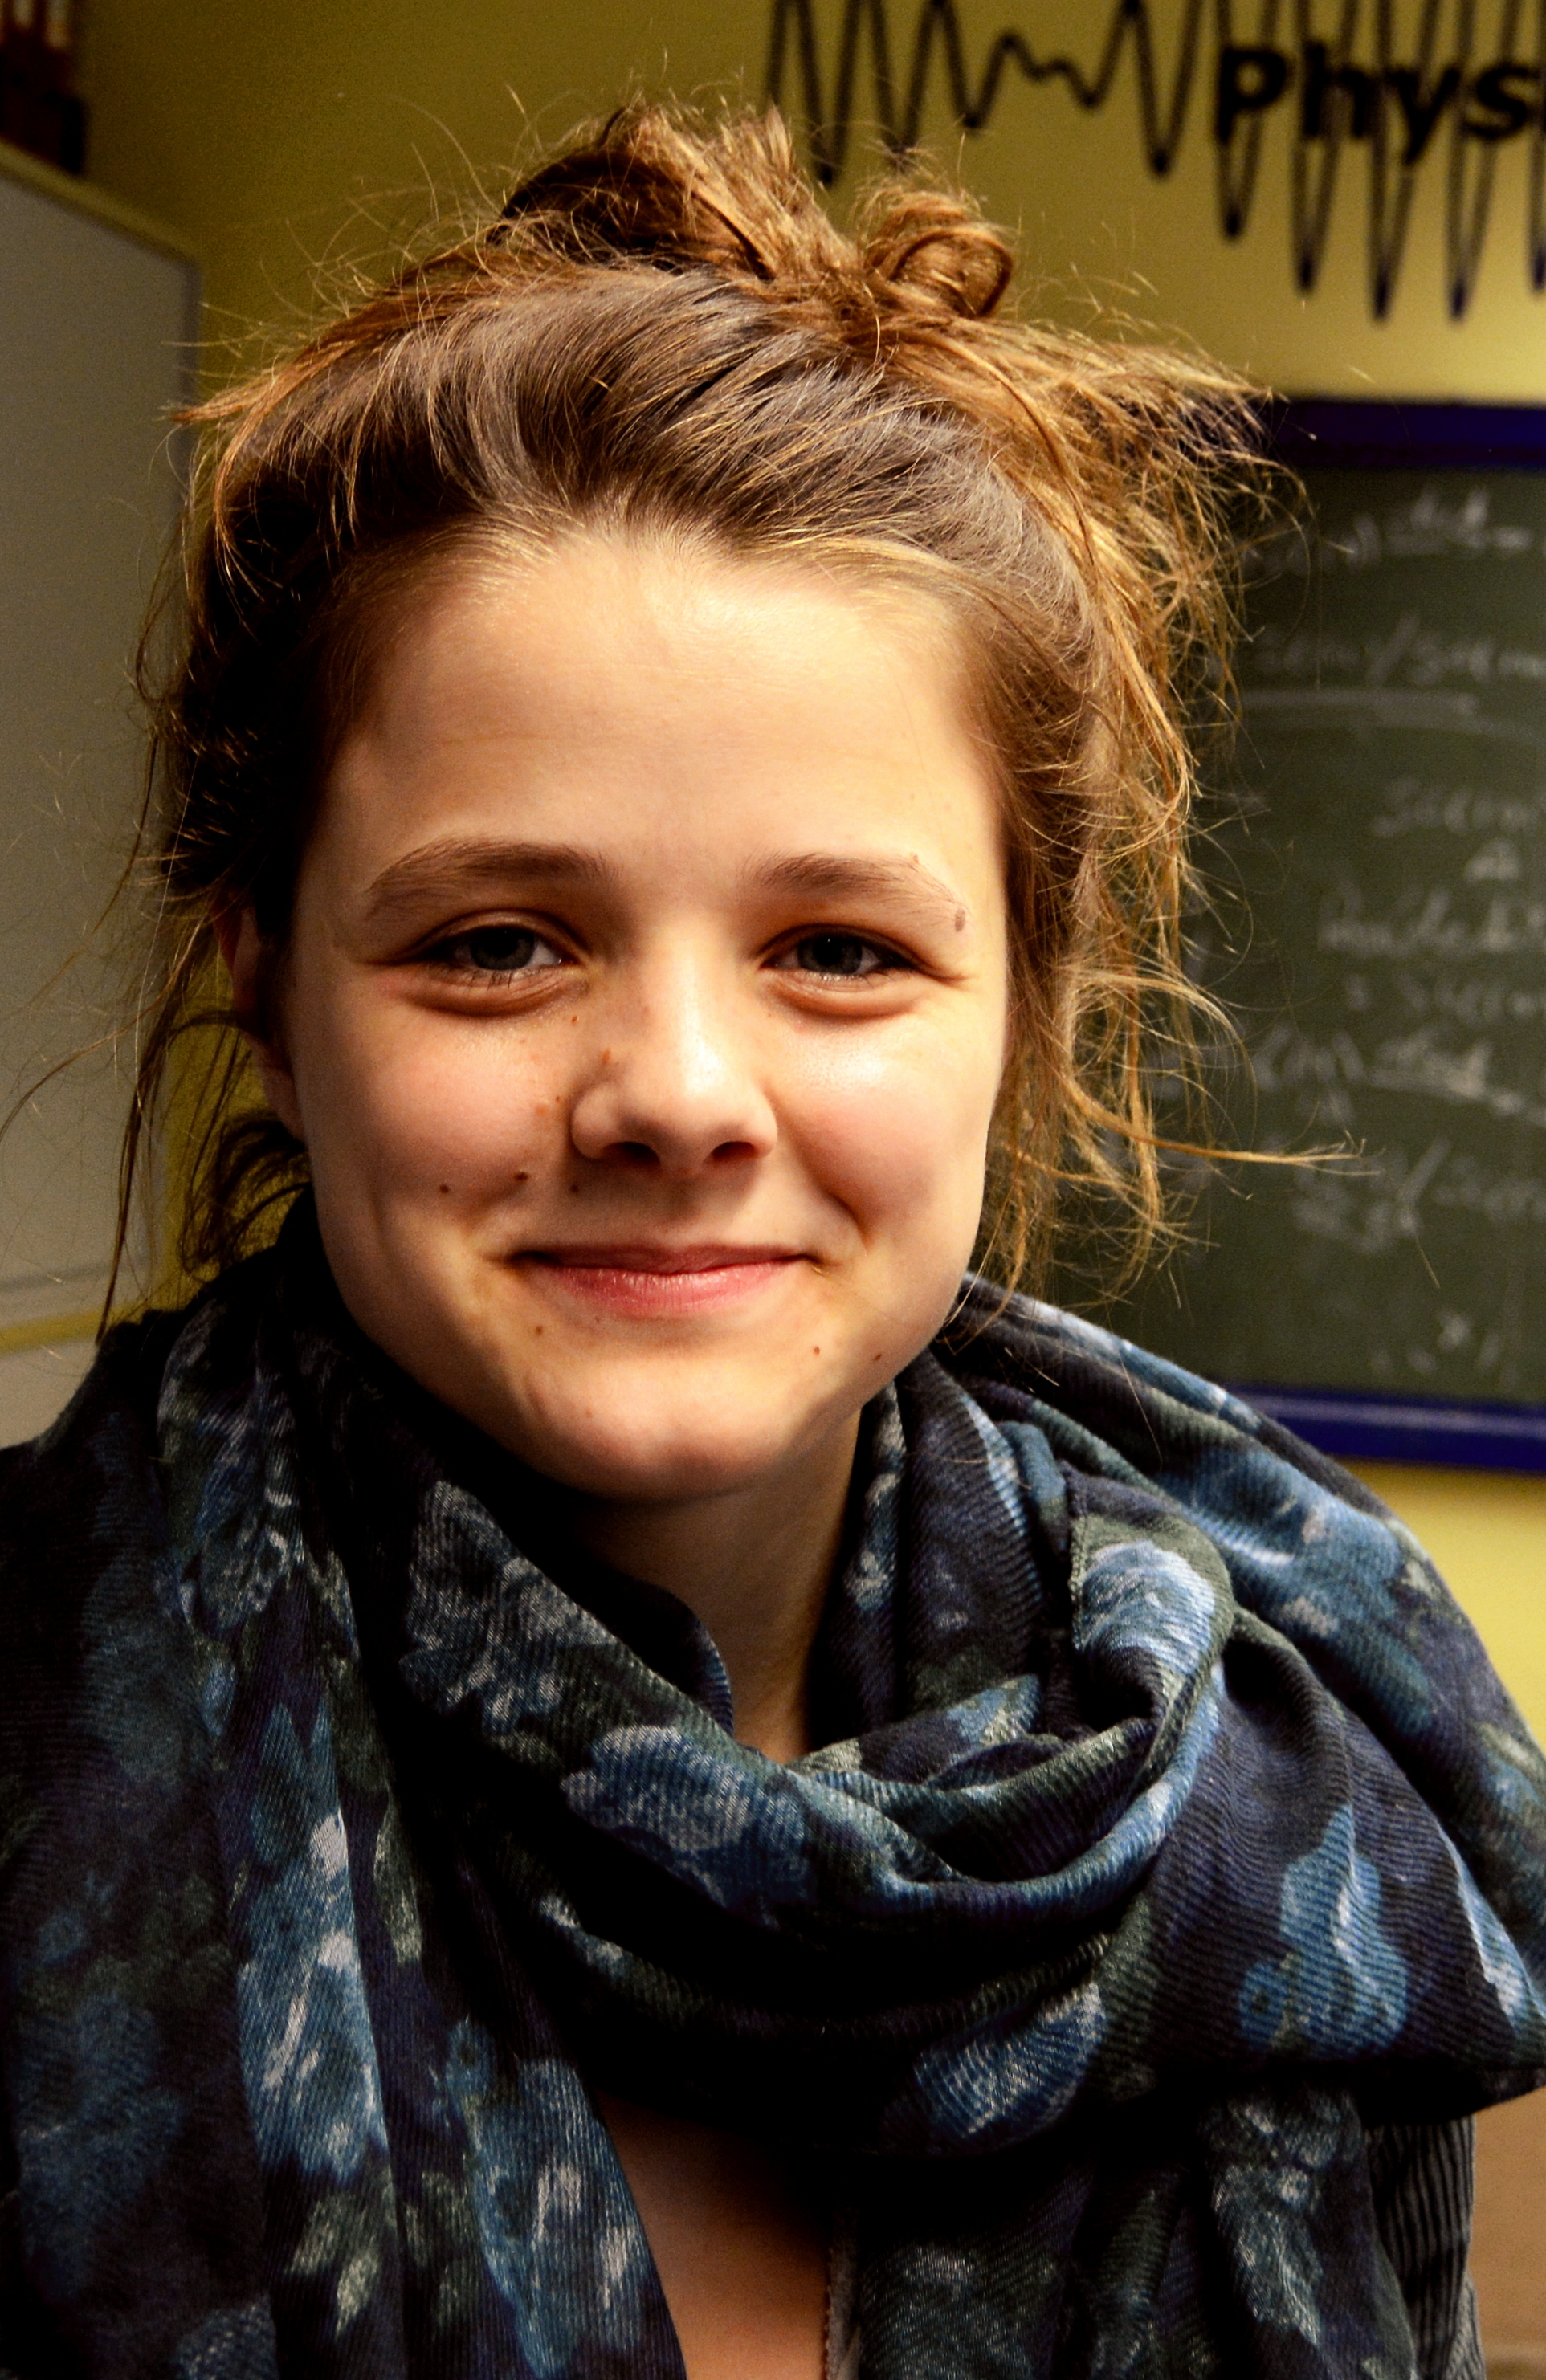
\includegraphics[width=\fibelstdlen]{res/vorstellungsfotos/pia_petrak_cropped.jpg}
	\end{wrapfigure}
}
{Hi, ich bin Pia, noch so gerade 22, und jetzt im dritten Mastersemester. Ich kümmere mich um den Bama-Tag. Da können alle Arbeitsgruppen Bachelor- und Masterarbeitsthemen vorstellen...Ansonsten will ich eigentlich nur noch los werden:
	Viel Spaß, vor allem in der O-Woche und hört bloß nicht auf mit Physik!
}
\vspace{\baselineskip}

\fibelvorstellung{
	\begin{wrapfigure}{l}{0cm}
		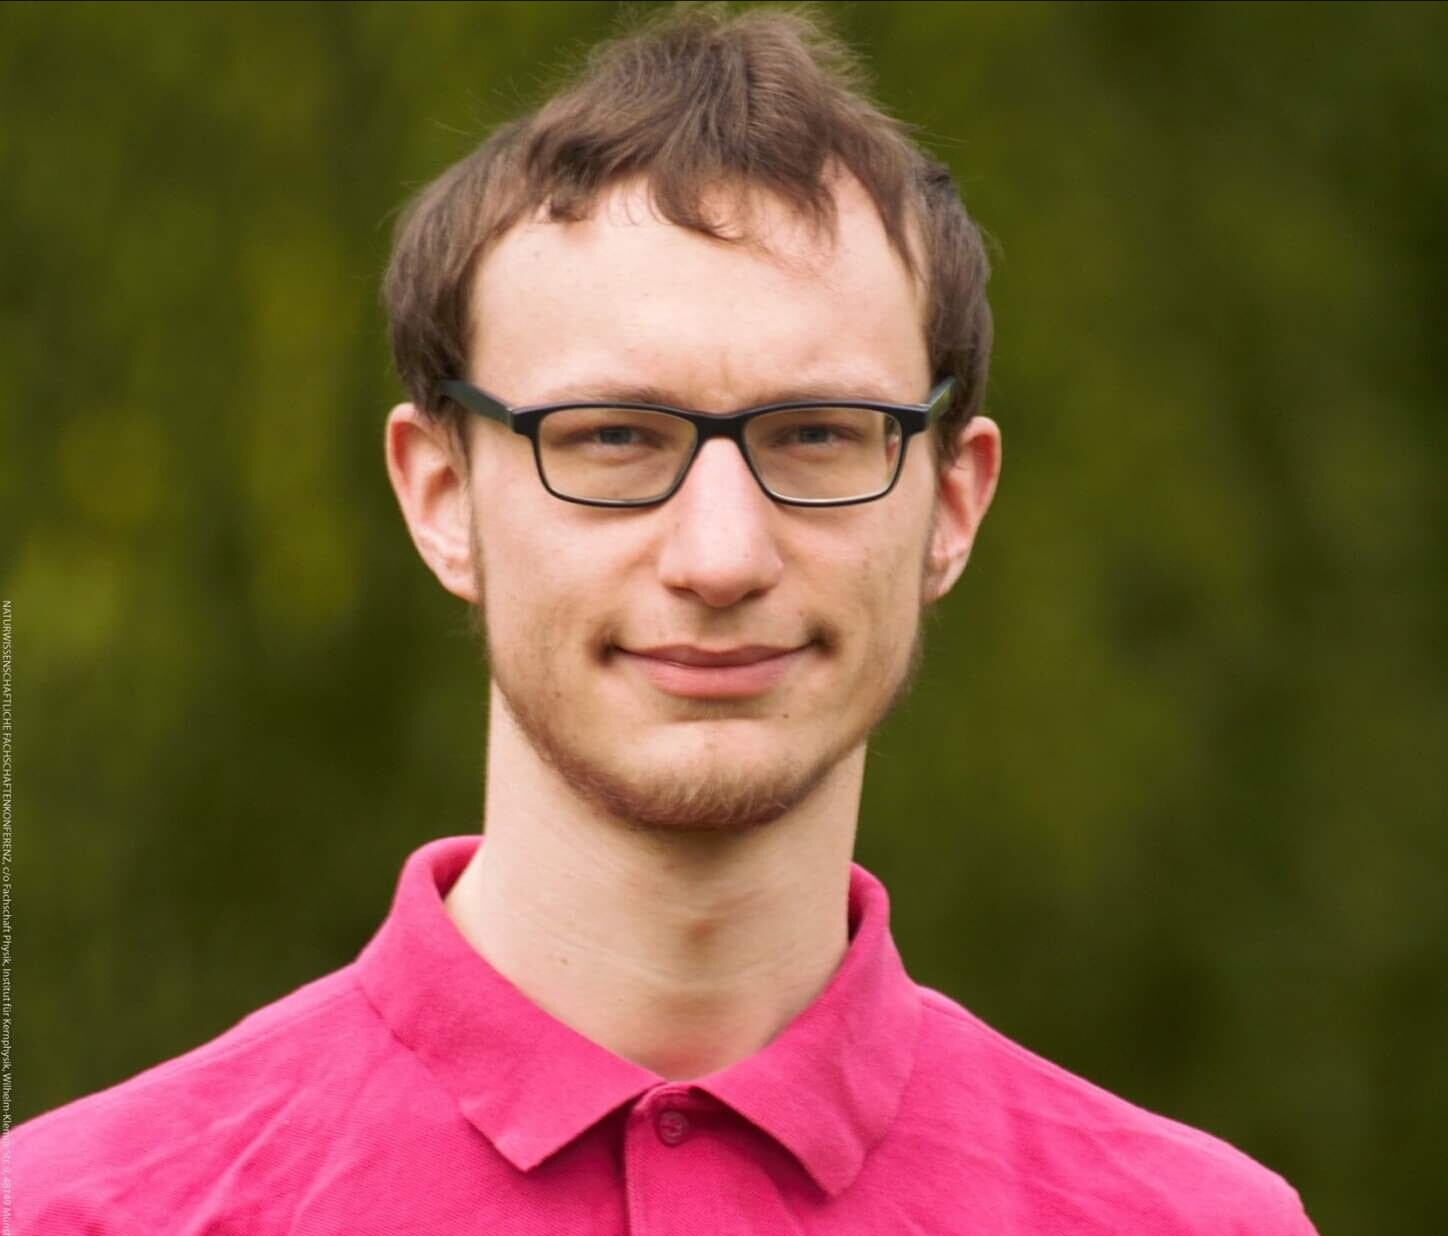
\includegraphics[width=\fibelstdlen]{res/vorstellungsfotos/michael_te_vrugt}
	\end{wrapfigure}
}
{Hi, ich bin Michael und beginne gerade mit meiner Promotion. In der Fachschaft bin ich als Vorsitzender, Beauftrager für alles mögliche, Mitglied des O-Wochen-Teams sowie diverser Gremien immer gerne dabei. Bei Fragen zu Philosophie, einem Doppelstudium, Auslandsjahr oder Stipendium - oder natürlich auch allem anderen - seid ihr bei mir genau richtig. Ansonsten wünsche ich euch viel Spaß in der O-Woche, und vielleicht sieht man sich ja mal bei einer Fachschaftssitzung :)}

\fibelvorstellung{
	\begin{wrapfigure}{r}{0cm}
		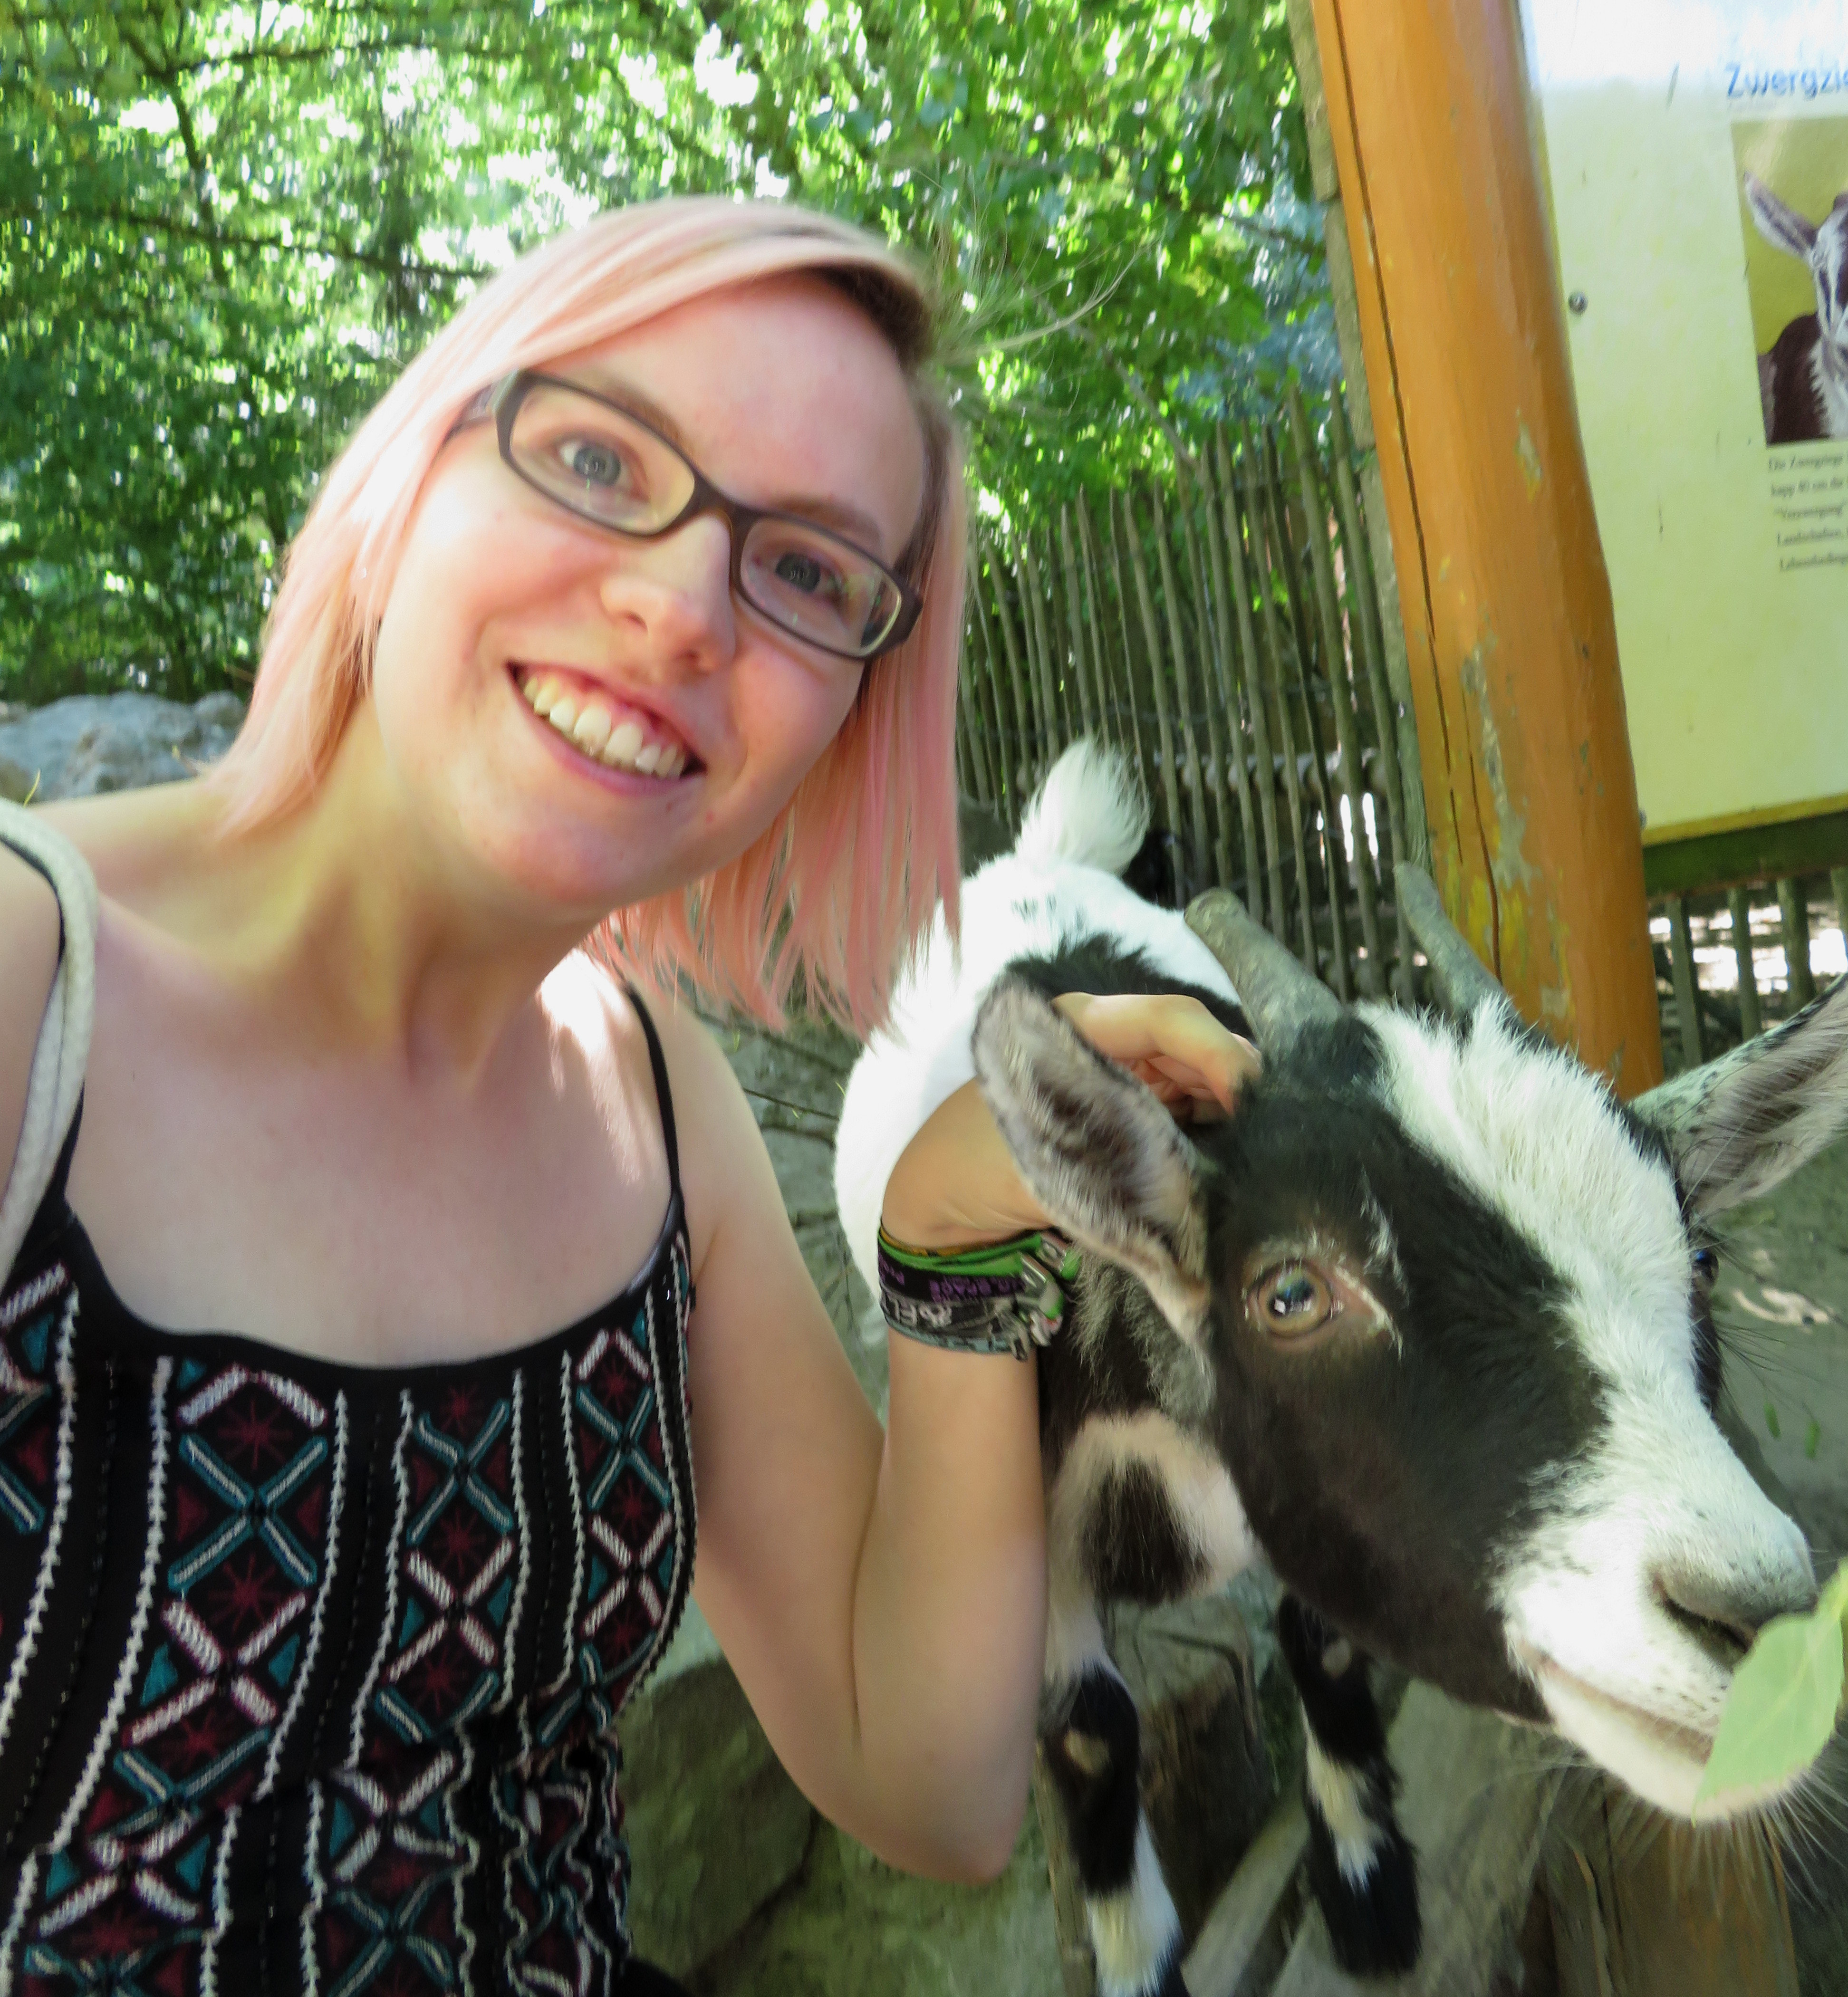
\includegraphics[width=\fibelstdlen]{res/vorstellungsfotos/miriam_neumann_cropped.jpg}
	\end{wrapfigure}
}
{Hey, ich bin Miri, 23 und gerade mitten in meinem Master. Bei einem Tee (oder Bier ;)) könnt ihr mich gerne über das Studium oder die Stadt ausfragen. Auch falls ihr sonst etwas wissen wollt, Hilfe braucht oder einfach nur quatschen wollt, seit ihr willkommen! Man erkennt mich am rosa Haar (oder anderen Farbexperimenten) :-)}

\fibelvorstellung{
	\begin{wrapfigure}{r}{0cm}
		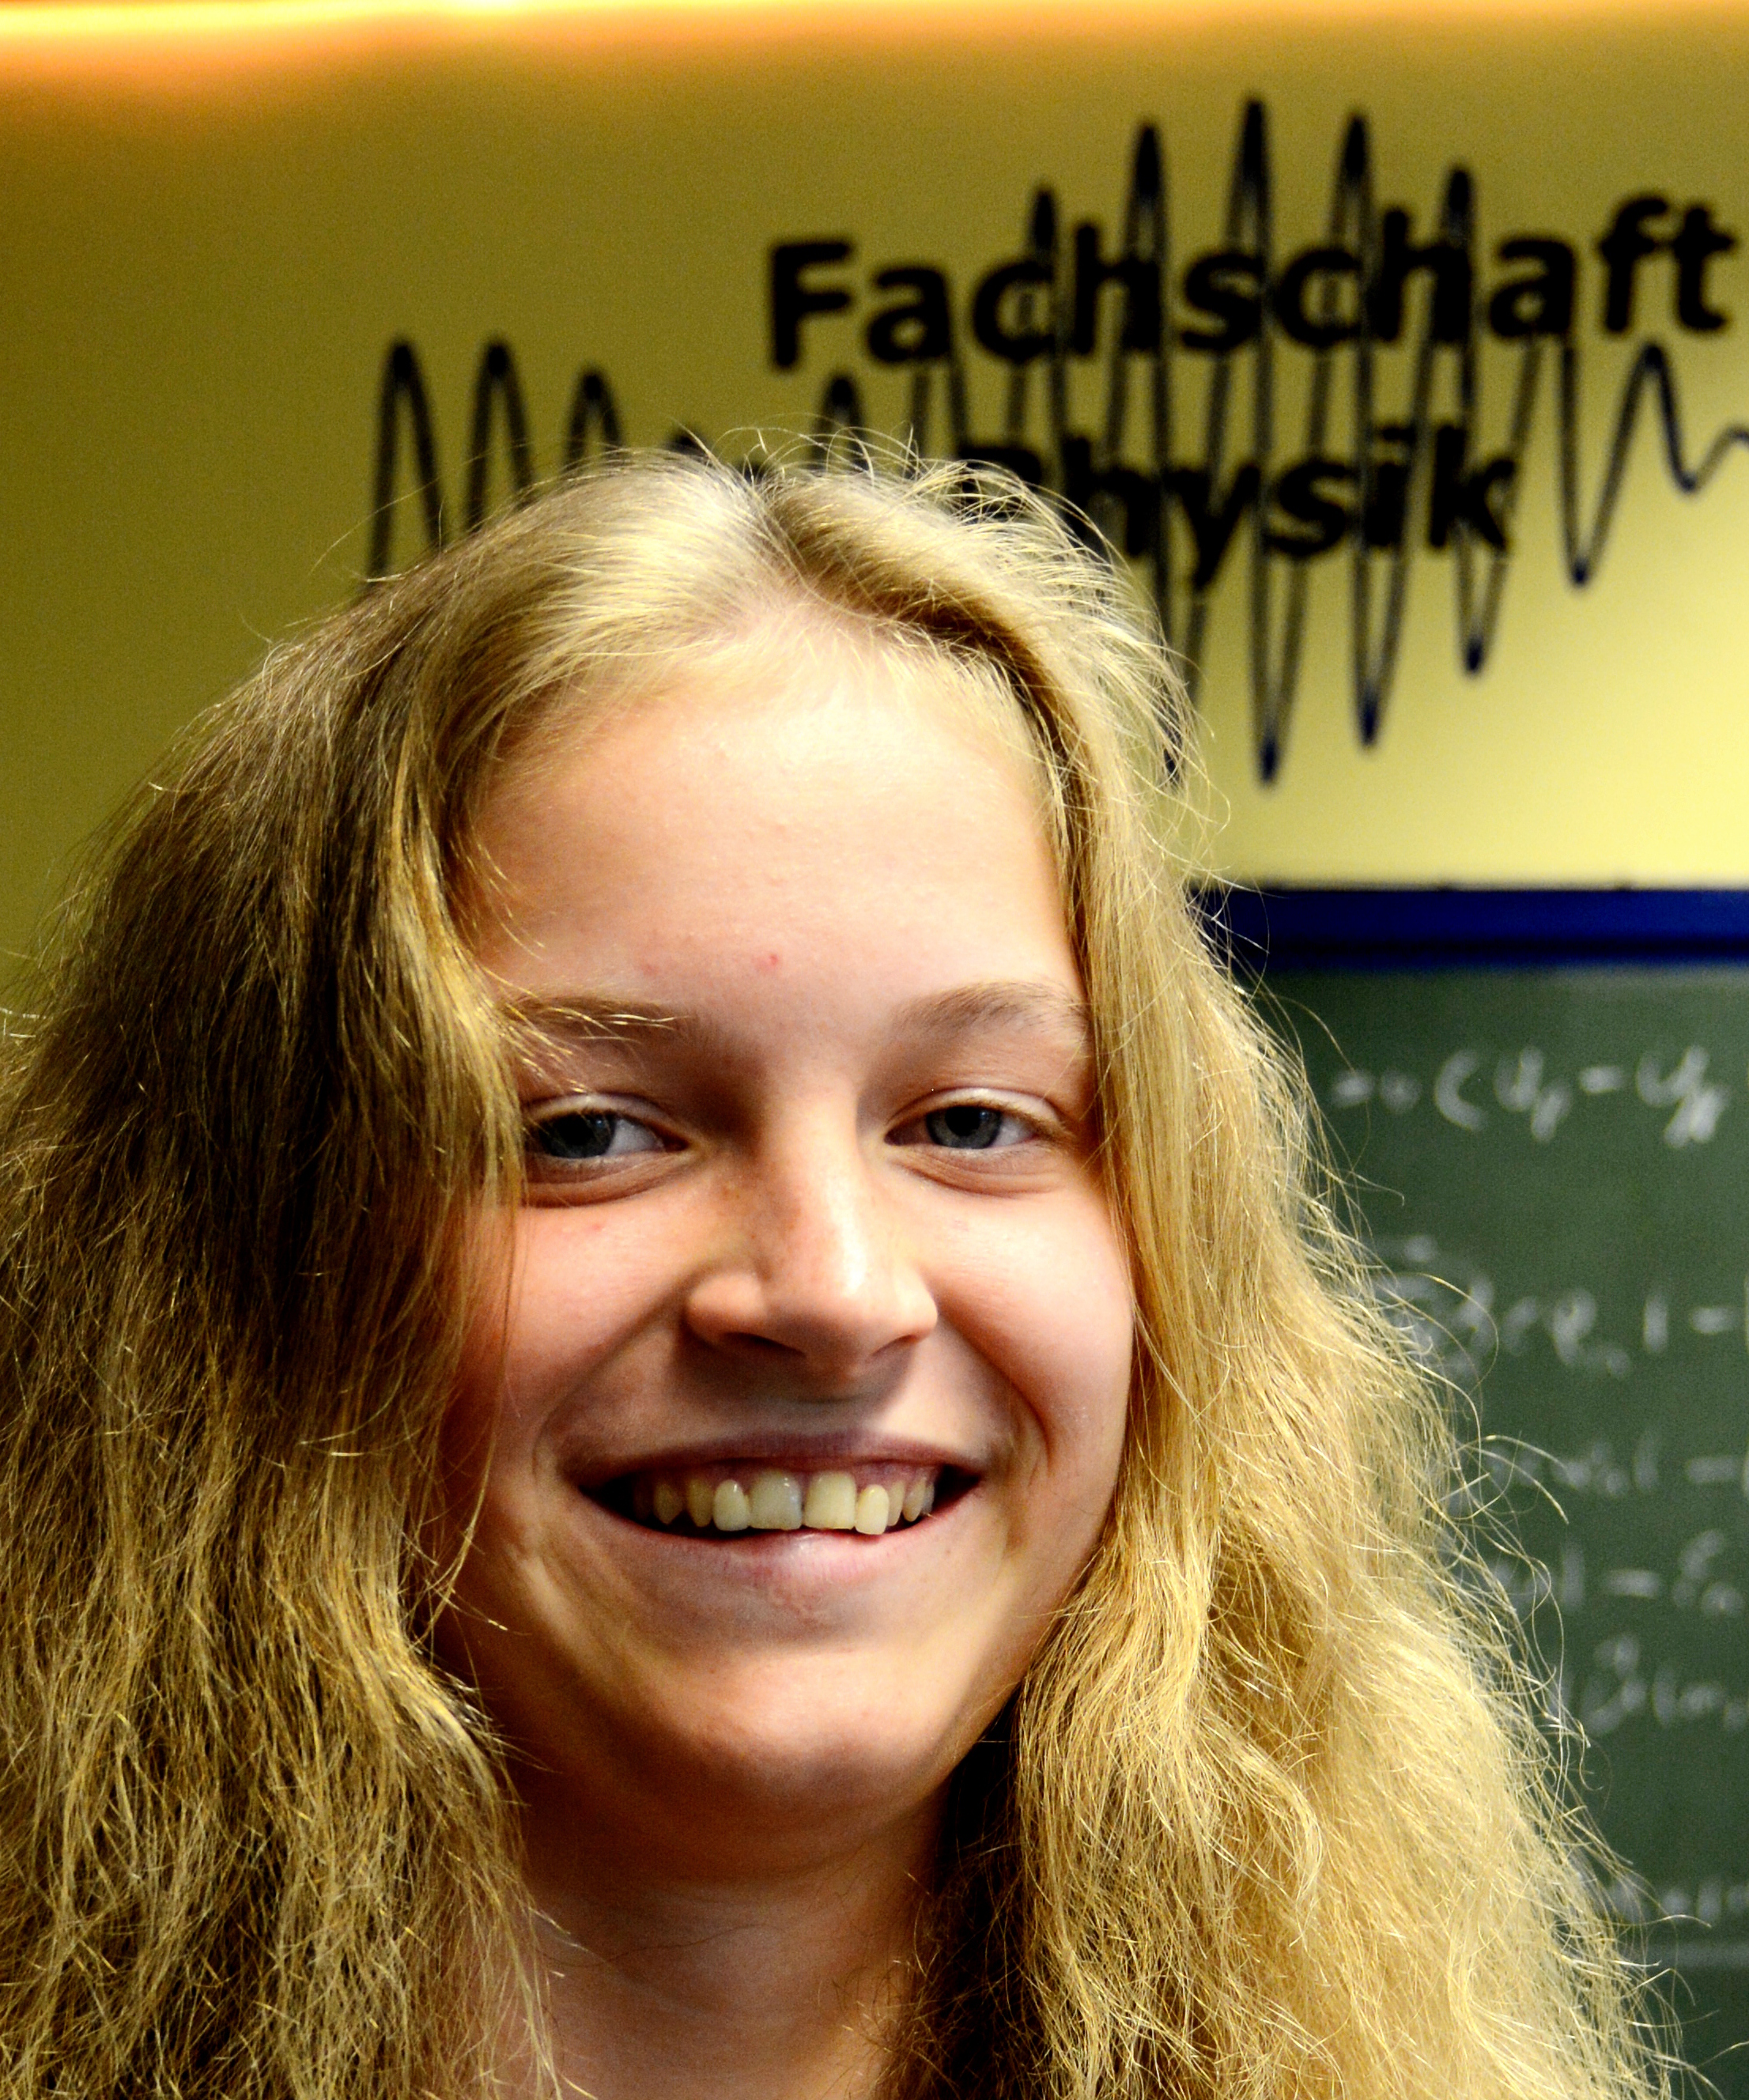
\includegraphics[width=\fibelstdlen]{res/vorstellungsfotos/johanna_jakob_cropped.jpg}
	\end{wrapfigure}
}
{Moin! Ich bin Johanna und bin inzwischen im zweiten Masterjahr. In der Fachschaft bin ich von Anfang an dabei.
}
\vspace{3\baselineskip}


\fibelvorstellung{
	\begin{wrapfigure}{l}{0cm}
		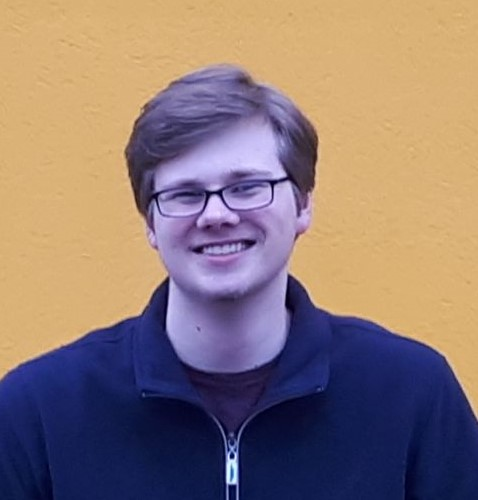
\includegraphics[width=\fibelstdlen]{res/vorstellungsfotos/joern_sieveneck}
	\end{wrapfigure}
}
{Hi, ich bin Jörn und bin mittlerweile im 7. Semester Physik
	Ich bin zuständig für die Evaluation der Lehre und den LaTeX-Kurs.
	Auch bei anderen Fragen könnt ihr euch gerne an mich wenden.}

\fibelvorstellung{
	\begin{wrapfigure}{r}{0cm}
		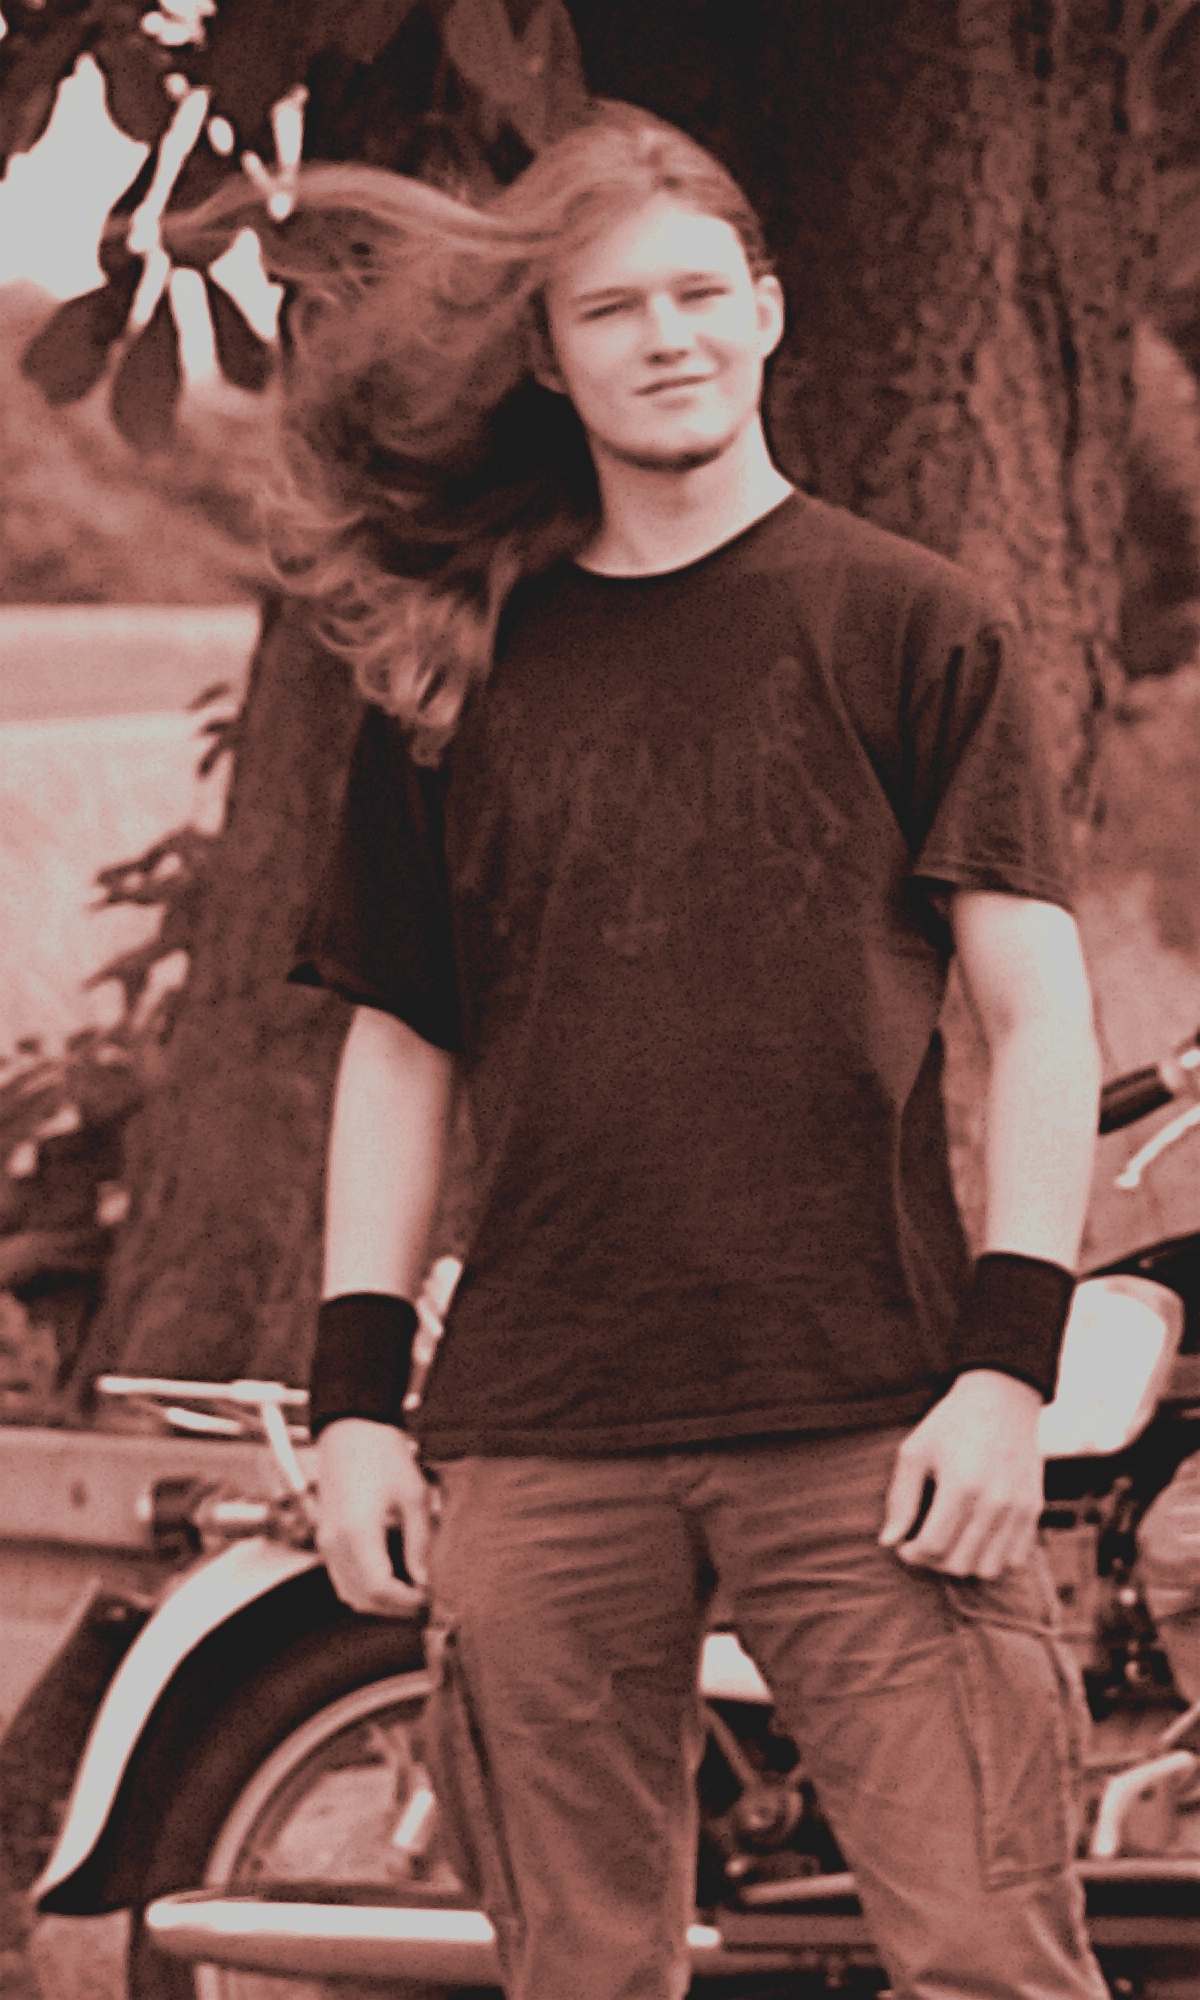
\includegraphics[width=\fibelstdlen]{res/vorstellungsfotos/jan_honermann}
	\end{wrapfigure}
}
{Hi, ich bin Jan und sitze gerade an meiner Doktorarbeit. Falls ihr Fragen habt, könnt ihr euch gerne an mich wenden, ich bin meistens netter, als ich aussehe ;)
}

\fibelvorstellung{
	\begin{wrapfigure}{l}{0cm}
		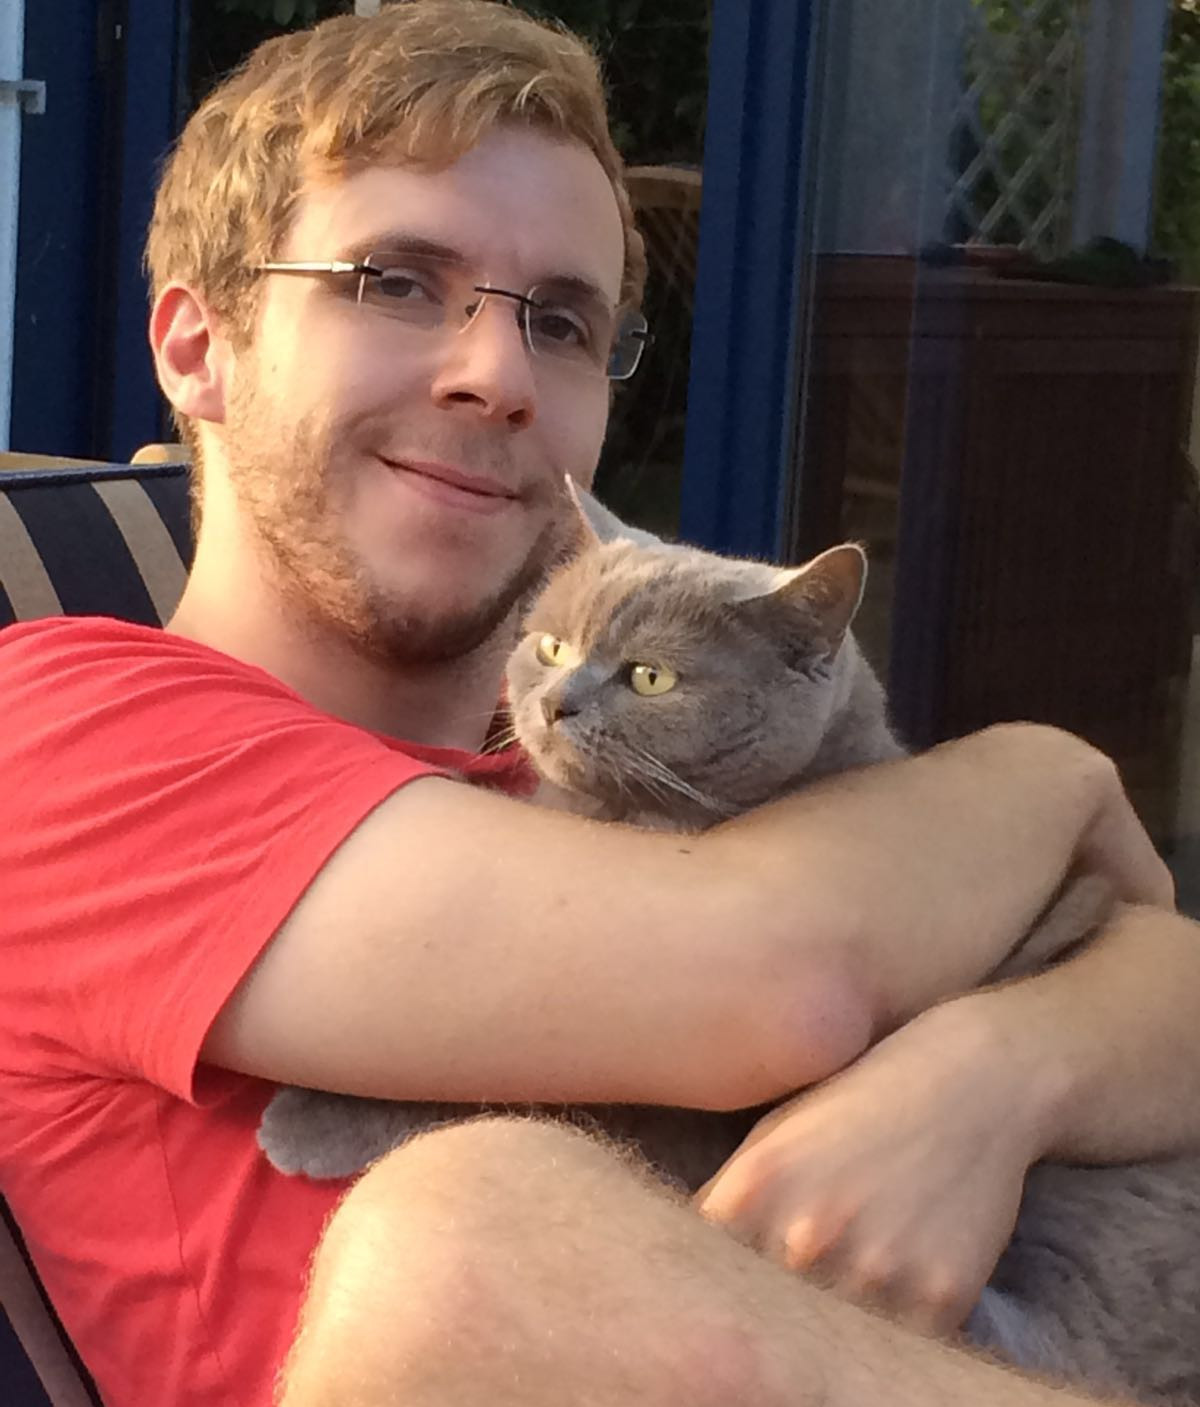
\includegraphics[width=\fibelstdlen]{res/vorstellungsfotos/lukas_eschmann_cropped.jpg}
	\end{wrapfigure}
}
{Moin liebe Erstis,
	mein Name ist Lukas und schon seit 2012 in der Fachschaft. Mein "normales" Studium habe ich bereits abgeschlossen, kann also so ziemlich alle Fragen zum Studium beantworten.
	Ich bin mittlerweile im Promotionsstudiengang angekommen und bin nur noch wenig in Hörsälen oder dem Fachschaftsraum anzutreffen.
	Auch Fragen zu Forschungsschwerpunkten der Uni oder aktuellen Themen der Forschung könnt ihr mir gerne stellen.}

\fibelvorstellung{
	\begin{wrapfigure}{r}{0cm}
		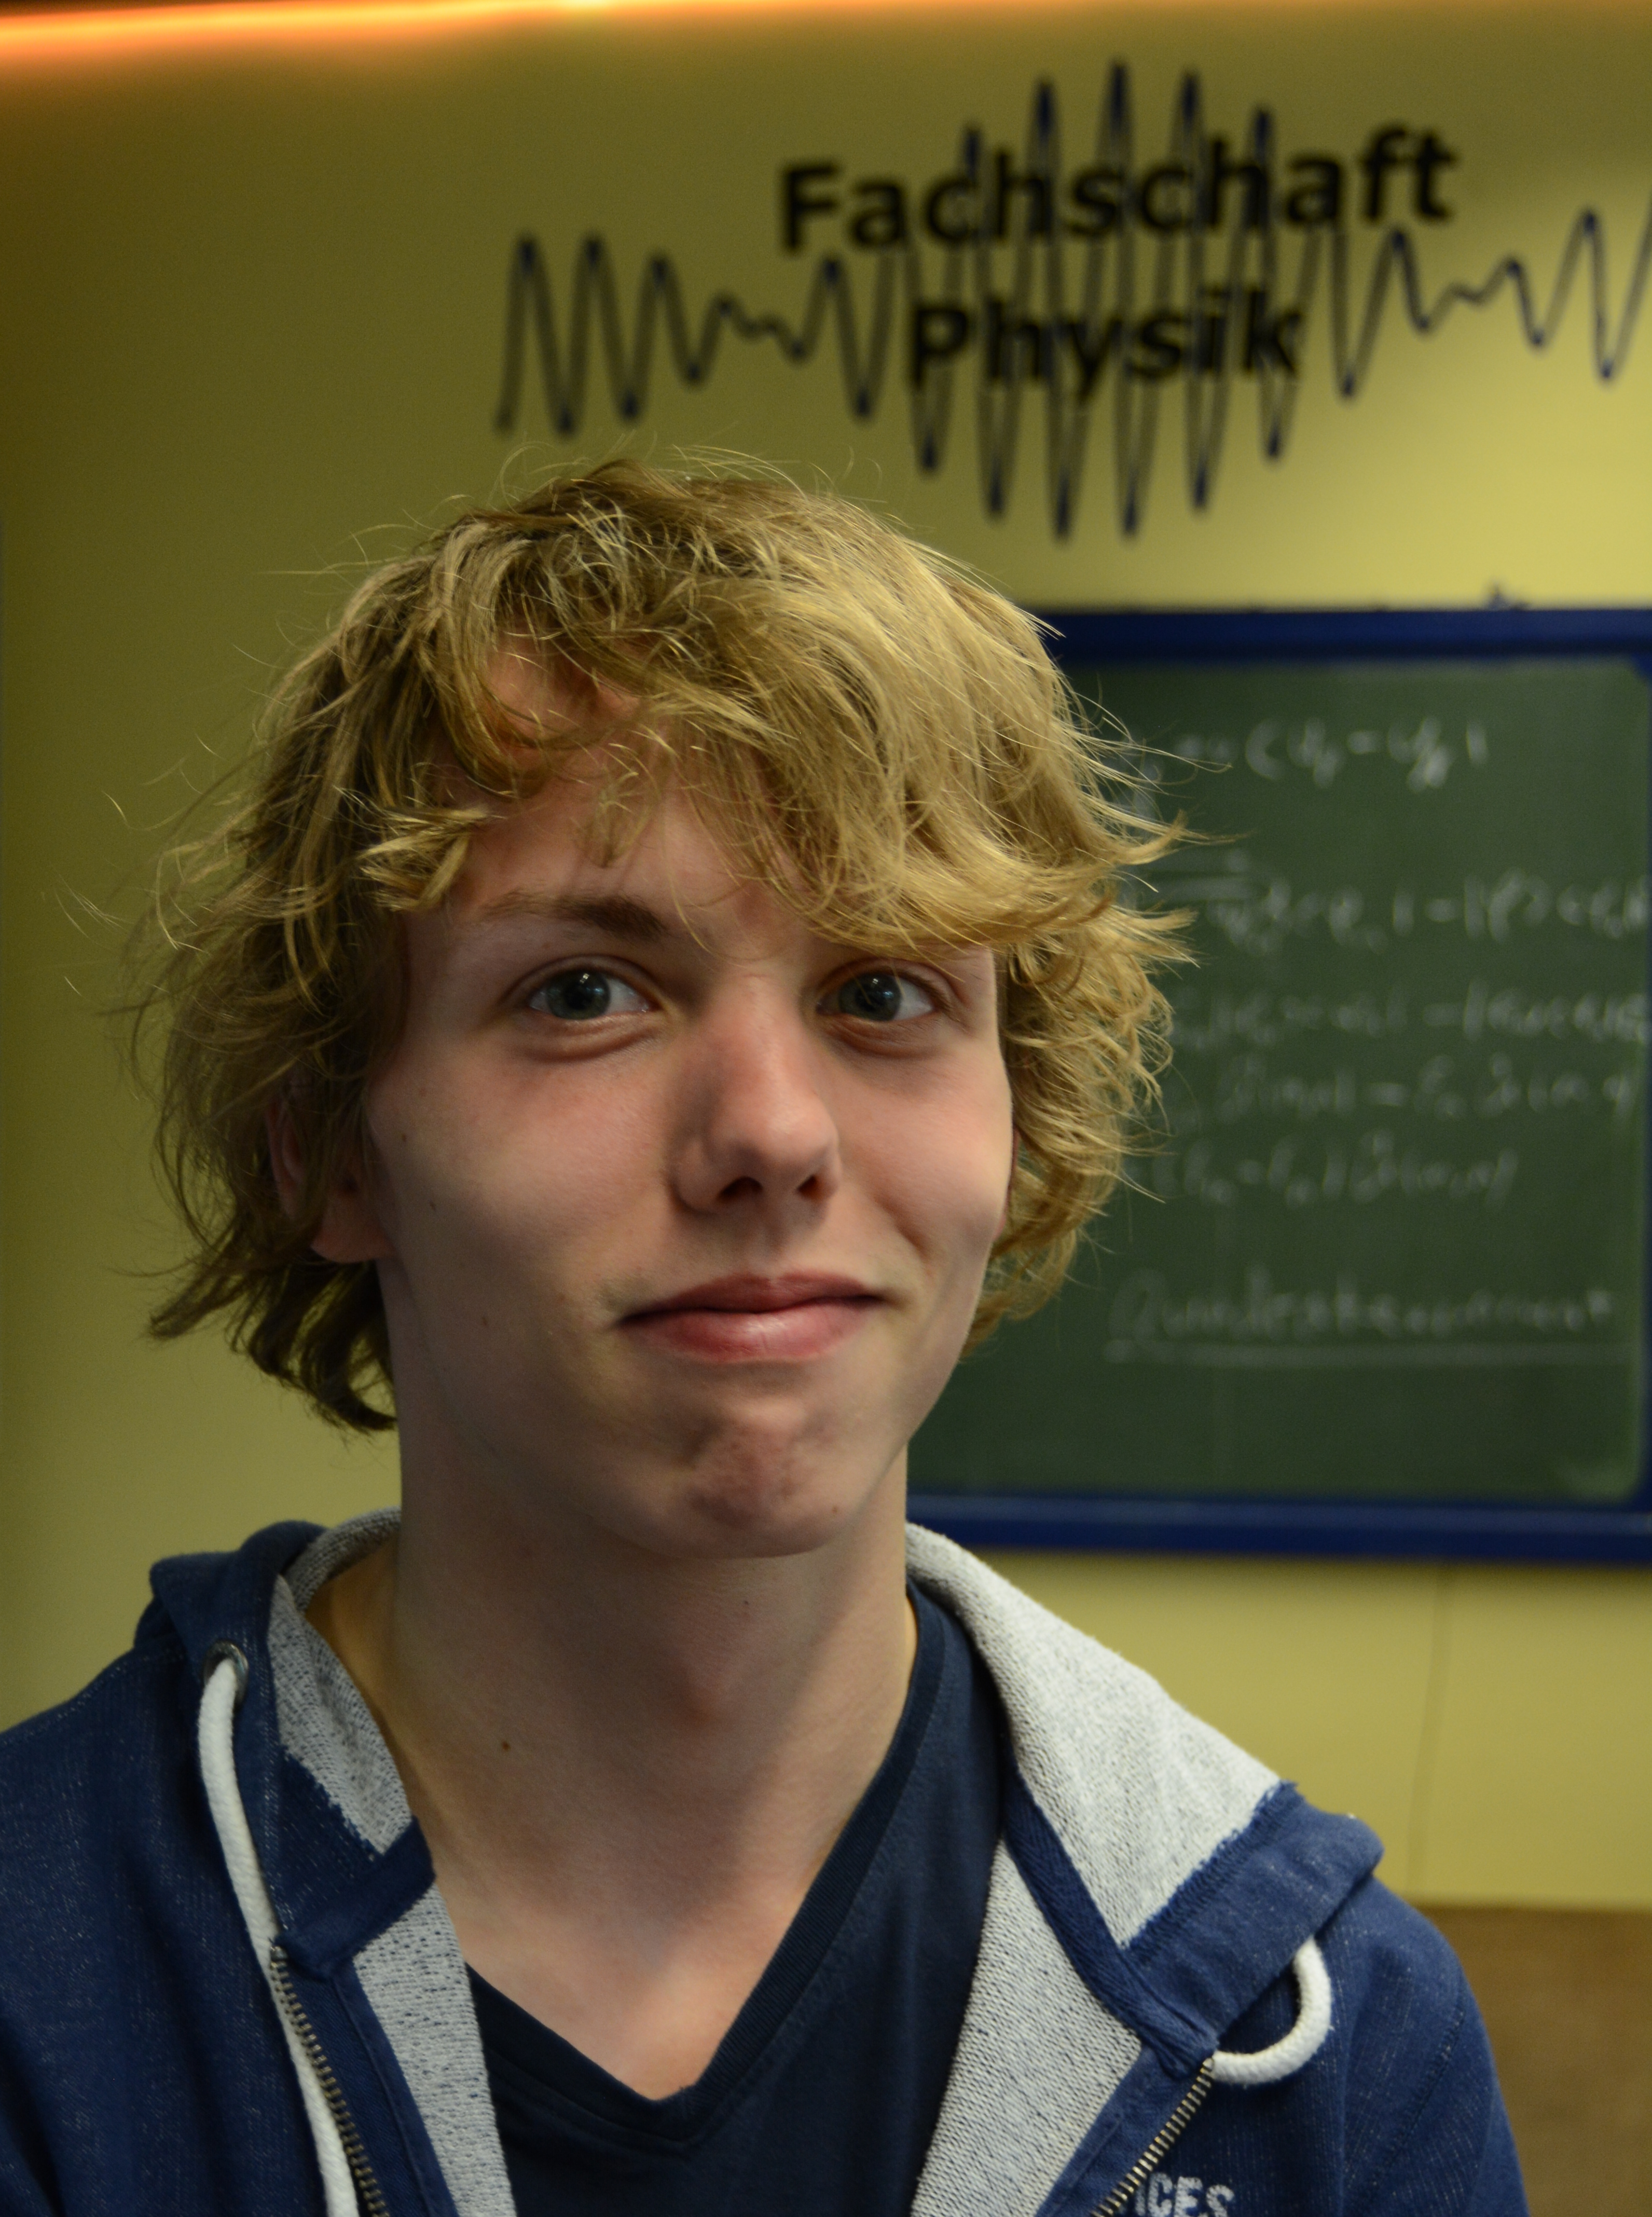
\includegraphics[width=\fibelstdlen]{res/vorstellungsfotos/marius_willer_cropped.jpg}
	\end{wrapfigure}
}
{Hi, ich bin Marius und heiße euch auch herzlich willkommen hier in Münster. Wenn ihr die Stadt noch nicht kennt, dann freut euch darauf, sie kennenzulernen. Das Studium wird zwar hart, aber lasst euch trotzdem nicht die Freude dran nehmen. ¡ Mucha suerte !}







	

	


%
% \begin{center}
% 	
\includegraphics[width=\columnwidth]{res/fsphys_logo.pdf}
% \end{center}
%
%
%

%\vspace{6ex}
%
%\fibelvorstellung{
%	\begin{wrapfigure}{r}{0cm}
%		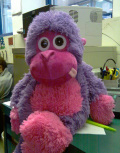
\includegraphics[width=\fibelstdlen]{res/vorstellungsfotos/fritz.png}
%	\end{wrapfigure}
%}
%{Hallo, ich bin Fritz und bin neu in der Fachschaft Physik.
%Die Mannschaft hier ist echt genial aufgestellt, sodass es richtigen Spaß macht, ein aktiver Teil der Universität Münster zu sein.
%Ich kann dir nur empfehlen: Mach' mit und verändere die Uni!}
\end{multicols}

